% Created 2022-01-11 Tue 11:11
% Intended LaTeX compiler: xelatex
\documentclass[11pt,landscape]{article}
\usepackage{graphicx}
\usepackage{longtable}
\usepackage{wrapfig}
\usepackage{rotating}
\usepackage[normalem]{ulem}
\usepackage{amsmath}
\usepackage{amssymb}
\usepackage{capt-of}
\usepackage{hyperref}
\usepackage[newfloat]{minted}
\usepackage{color}
\usepackage{listings}
\usepackage[top=2cm,bottom=2cm,right=2cm,left=2cm,landscape]{geometry}
\usepackage{multicol}
\usepackage{enumitem}
\usepackage{fancyhdr}
\setlist{noitemsep}
\setlength{\parindent}{0pt}
\setlength{\columnseprule}{0.2pt}
\author{Olivier Lischer}
\date{\today}
\title{AIFo Summary}
\hypersetup{
 pdfauthor={Olivier Lischer},
 pdftitle={AIFo Summary},
 pdfkeywords={},
 pdfsubject={},
 pdfcreator={Emacs 27.2 (Org mode 9.5.1)}, 
 pdflang={English}}

\pagestyle{fancy}
\fancyhf{}
\fancyhead[R]{AIFo-HS21}
\fancyhead[L]{Exam Summary}
\fancyfoot[CE,CO]{\leftmark}
\fancyfoot[R]{\thepage}
\fancyfoot[L]{Olivier Lischer}

\begin{document}

\begin{multicols}{3}

\textbf{Keywords}

\begin{itemize}
\item \emph{predictive model}: the goal is to find a model that performs well on new / unseen data
\item \emph{new / unseen data}: data which the model did not seen during the training
\item \emph{(low) generalization error}: if the predicitve model has low generalization error it performs well on new / unseen data
\item \emph{test-error / out-of-sample error}: test-error is an estimate of the generalization error (splitting data in training- and test set - calculate error on test set). can be splited in to bias / variance.
\item \emph{bias}: simple models -> high bias (low variance). There is a risk of undertiffnt
\item \emph{variance}: complex models -> small bias (high variance). There is a risk of overfitting
\item \emph{underfitti}:ng
\item \emph{overfitti}:ng
\item \emph{regularization}: is a method to control the model complexity. Using regularization we can find the optimal balance in the bias-varance trade-off
\item \emph{bias-variance trade-of}:f
\item \emph{L1 / L2 norm}: Penalty for model complexity
\end{itemize}

\textbf{Machine Learning Types}

\begin{itemize}
\item \href{../../../roam/20210924090800-unsupervised_learning.org}{Unsupervised learning}
\item \href{../../../roam/20210924091334-supervised_learning.org}{Supervised learning}
\item \href{../../../roam/20210924091935-reinforcement_learning.org}{Reinforcement learning}
\end{itemize}

\textbf{NLP}

Natural Language Processing is a sub-field of artificial intelligence.
It aims to understand and generate human (natural) language.
NLP is often used in Chats Bots.

\textbf{Dialogflow}

\begin{itemize}
\item Intent matching: \href{https://www.youtube.com/watch?v=9aHusGxntPw}{Dialogflow Intents: Know what your users want}
\item Dialogflow Entities: \href{https://www.youtube.com/watch?v=kzdL6GxJ\_WY}{Dialogflow Entities: Identify things your users mention}
\item Dialog Control: \href{https://youtu.be/-tOamKtmxdY}{Dialogflow Dialog Control: Shape the flow of your conversation}
\end{itemize}



\textbf{The 4 Ingredients of Machine Learning}

\begin{enumerate}
\item \emph{Data}:
\begin{itemize}
\item Sometimes you have to do some clean up or some normalization
\item we can not do better than what is in this data
\end{itemize}
\item \emph{Cost-Function (loss)}:
\begin{itemize}
\item a formal (mathematical) expression for "good" / "bad"
\item \href{../../../roam/20211004175550-mean_squared_error.org}{Mean Squared Error} is commonly used
\end{itemize}
\item \emph{Model}:
\begin{itemize}
\item Something to map input to the output
\item two parameter linear / complicated neural network
\end{itemize}
\item \emph{Optimization Procedure}:
\begin{itemize}
\item An algorithm that changes the parameters of the model such that the cost function is minimized.
\end{itemize}
\end{enumerate}

+3 Steps for better ML:
\begin{enumerate}
\item Performance optimization: Building efficient pipe-lines is difficult
\item Visualization and evaluation of the learning Process: Learning curves, Performance Measures
\item Cross-Validation \& Regularization: goal to develop models that generalize
\end{enumerate}

\textbf{One-Hot Representation}

One-Hot is possible way to represent words as vectors.
The number of diffrent words is the dimension of the vector.
Each word has now only set one possition to 1.

Problems with this approach are:
\begin{itemize}
\item the vectors are very hight dimensional
\item is not memory efficient, a single 1 and for example 99'9999 zeros
\item no generalization possible. This representation can not store the meaning of a word
\end{itemize}


\textbf{Index Representation}

Index is a \emph{dense equivalent} to \href{../../../roam/20211004181318-one_hot_representation.org}{One-Hot Representation}.
Each word is asigned an index.
Indexing is often used as preprocessing step.


\textbf{Distributed Representation}

\begin{center}
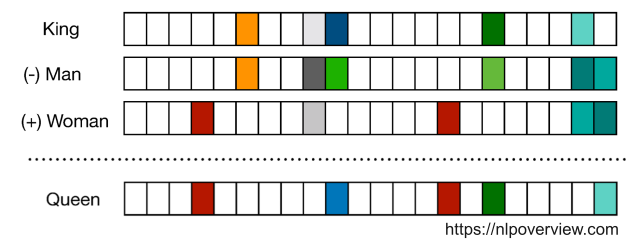
\includegraphics[width=.9\linewidth]{img/distributed_representation.png}
\end{center}


\textbf{Word Embedding}

A Word embedding is something like a function / black box which maps a word to a vector \vec{v}.


\textbf{Cosine Similarity}

The cosine similarity is just the formula for the \href{../../../roam/20211004182731-dot_product.org}{Dot Product} transformed:
$$
\cos(\phi) = \frac{A \cdot B}{|A||B|}
$$

\textbf{Coseine distance}:

\begin{align}
\text{cosine distance} &= 1 - \text{cosine similarity} \\
&= 1 - \frac{A \cdot B}{|A||B|}
\end{align}

\textbf{Probability}

The marginal probability is the general known probabiliy.

The Joint Probaility \(p(x, y)\) means that the event x and the event y occurs. If x and y are independent the formula is:
$$
p(x,y) = p(x) \cdot p(y)
$$

If x and y are \textbf{not} independent then the formula is:
$$
p(x,y) = p(x|y) \cdot p(y)
$$

\textbf{Conditional Probability}

$$
P(Y|X) = \frac{P(Y \cap X)}{P(Y)}$
$$


\textbf{Bayes Rule}

$$
P(Y|X) = \frac{P(X|Y) \cdot P(Y)}{P(X)}
$$

\textbf{Regression}

Linear Regression is a \href{../../../roam/20210924091334-supervised_learning.org}{Supervised learning} algorithm.


\textbf{MSE}

\begin{align}
E &= \frac{1}{2N} \sum_{i=1}^N e_i^2 \\
&= \frac{1}{2N} \sum_{i=1}^N (y_i - (a \cdot x_i + b))^2
\end{align}

\textbf{Residual}

The Residual \(e\) is the difference between the original \(y_i\) and the estimated \(\hat{y_i}\).


\textbf{Bias}

The inability for a machine learning methods (e.g. Linear Regression) to capture the true relationship is called bias.

\textbf{Variance}

The difference in the fits between training and testing data.


\textbf{Gradient Descent}

Gradient Descent is an algorithm used for optimization problems.
It works with an iterative approach using gradients. 
On each iteration the error function is derived.

\textbf{SGD}

The Stochastic Gradient Descent (SGD) is a variant of \href{../../../roam/20211208163604-gradient_descent.org}{Gradient Descent}.
Instead of calculating the Update Rule (\href{../../../roam/20211208163727-the_gradient_descent_update_rule.org}{The Gradient Descent Update Rule}) for all available data only one random chosen data is used.
SGD is therefore a \href{../../../roam/20211208163604-gradient_descent.org}{Gradient Descent} with Batch Size 1 (\href{../../../roam/20211208170338-the_batch_size_in_sgd.org}{The batch-size in SGD}).
Since you only use a subset, it is faster, but you might not find the global minimum.

\textbf{Batch Size}

The subset of the data which are used for Gradient Descent (\href{../../../roam/20211208163604-gradient_descent.org}{Gradient Descent}) is called \textbf{batch-size}.
Increasing the batch-size will reduce the variance of the gradient estimation.
There's no "best" batch-size, but often mini-batches of size \(n=32\) or \(n=64\) are used. 

\begin{itemize}
\item \emph{n = 1}: \href{../../../roam/20211208165153-the_stochastic_gradient_descent.org}{The Stochastic Gradient Descent}
\item \emph{1 < n < N}: mini-batches (an approx. gradient is used)
\item \emph{n = N}: the real gradient is used
\end{itemize}

\textbf{Update Rule}

\begin{equation}
  \begin{bmatrix}
    a \\
    b \\
  \end{bmatrix}_{t+1} 
  =    \begin{bmatrix}
    a \\
    b \\
  \end{bmatrix}_{t} - \alpha 
  \begin{bmatrix}
    \frac{\partial E}{\partial a} \\
    \frac{\partial E}{\partial b} \\
  \end{bmatrix} \Big\rvert _{\begin{bmatrix}
      a \\
      b \\
    \end{bmatrix}_{t} }
\end{equation}

\textbf{Derived MSE}

\begin{align}
  \textrm{E} &= \frac{1}{2N} \sum_{i=1}^{N} (y_i - (a \cdot x_i + b))^2 \\
  \frac{\partial \textrm{E}}{\partial a} &= \frac{1}{N} \sum_{i=1}^{N} (y_i - (a \cdot x_i + b)) (-x_i) \\
  &\approx \frac{1}{n} \sum_{j \in J_n} (y_j - (a \cdot x_j + b)) (-x_j)  \\
  \frac{\partial \textrm{E}}{\partial b} &= \frac{1}{N} \sum_{i=1}^{N} (y_i - (a \cdot x_i + b)) (-1) \\
  &\approx \frac{1}{n} \sum_{j \in J_n} (y_{j} - (a \cdot x_{j} + b)) (-1)  \\
\end{align}


\textbf{Annealed Learning}

In the Update Rule is the learning rate \(\alpha\) specified.
At the beginning the learning rate \(\alpha\) is high and over time the value is reduced.


\textbf{In-sample error}

The \emph{in-sample error}, also called \emph{training error}, is error which your model makes when predicting the sample data.
It is possible to find a model which fits perfectly the data.

\textbf{out-of-sample error}

When you try to predict with a model \emph{unseen} data the resulting error is called \emph{out-of-sample error}.
An other name is \emph{generalization error} or \emph{test error}.


\textbf{Bias-Variance Trade-off}

There is a trade-off: higher bias implies lower variance, lower bias implies higher variance.
Normally we want reduce the variance (no surprise with out-of-sample data)


\textbf{Regularization}

Regularization is used to punish single parameters of the model to prevent overfitting.
Normally the L1 and L2 Norms are used to measure the model complexity:
\begin{enumerate}
\item L1 - Norm \(\sum_i^p |\beta_i|\)
\item L2 - Norm \(\sum_i^p |\beta_i^2|\)
\end{enumerate}

\begin{equation}
  \sum_{i=1}^n(y_i - \sum_{j=1}^p x_{ij}\beta_j)^2 + \lambda \sum_{j=1}^p\beta_i^2
\end{equation}


\textbf{Cross-Validation}

To train your model you normally split your data in testing and training data.
If you create this split only once you can not verify how well your model performs on new data.
To solve this problem you can split your data in \(k\) times in \(k\) splits.
k-fold Cross-Validation is an implementation of Cross-Validation


\textbf{Hyper Parameters}

By "parameter" or "model parameter" we usually mean the weights of a model.
Parameters of the training procedure, (e.g. regularization parameter \(\lambda\)) are called hyper parameters.

\textbf{Neurons}

Artifical Nuerons are the building blocks for an ANN.
An Neuron receives an input vector (\([x_1 \; x_2 \; \ldots]\)).
Each input has a different \emph{weight} (\([w_1 \; w_2 \; \ldots]\)) and bias b (=intercept).
The neuron iteself:
\begin{enumerate}
\item calculates the sum of the weighted input (\(\vec{x} \cdot \vec{w}\))
\item adds a bias \(b\)
\item pass it through a nonlinear activation function (e.g. \href{../../../roam/20211214121924-relu.org}{ReLU})
\end{enumerate}


\textbf{ANN}

An ANN (Artifical Neural Network) consists of many \href{../../../roam/20211214121841-artifical_neurons.org}{Artifical Neurons}.
Basically the ANN is just a data-structure to define arbitrarily complex mathematical functions.
The ANN has 3 types of layer:
\begin{itemize}
\item one input layer
\item one or many input layers
\item one output layer
\end{itemize}


\textbf{Train ANN}

\begin{enumerate}
\item initial each weight randomly
\item on optimizer reduces a cost-function (e.g. \href{../../../roam/20211004175550-mean_squared_error.org}{MSE})
\begin{itemize}
\item for each weight the partial derived is calculated
\item Backpropagation is used to optimized the weigts (trains the \href{../../../roam/20211214110732-ann.org}{ANN}, used in Keras)
\end{itemize}
\end{enumerate}

\textbf{Classification}

Using classification you try to classify given data (X).

\textbf{sigmoid}

\begin{equation}
  sigmoid(y) = \frac{1}{1 + e^{-y}}
\end{equation}

\begin{align}
  y &= w_1x_1 + w_2x_2 + \cdots + w_nx_n \\
  sigmoid(y) &= \frac{1}{1 + e^{-y}}
\end{align}


\textbf{Train classification}

You have to minimize the cost by adjusting the weights.
This is called \textbf{Maximum Likelihood}.
We want to minimize the equation \ref{eq:org7858a22}.
This could be done with \href{../../../roam/20211208163604-gradient_descent.org}{Gradient Descent}.

\begin{equation}
\label{eq:org7858a22}
  \frac{-1}{N}\sum_{i=1}^{N}(y_i \cdot \log(p_i) + (1 - y_i)\cdot \log(1-p_i))
\end{equation}

The loss depends on prediction and reality:
\begin{itemize}
\item if I say it is very likely that it happens and it happens \(\rightarrow\) small loss
\item if I say it is very likely that it happens and but it does NOT happens \(\rightarrow\) big loss
\end{itemize}

\begin{center}
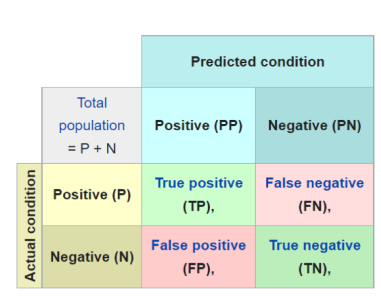
\includegraphics[width=.9\linewidth]{img/confusion_matrix.png}
\end{center}


\textbf{Mean Accuracy}:

How often is the classifier correct?
\begin{equation}
Accuracy = \frac{t_p + t_n}{n}
\end{equation}

\textbf{Mean Error}:

How often is the classifier wrong?
\begin{equation}
Error = \frac{f_p + f_n}{n}
\end{equation}

\textbf{Precision}:

When the prediction is 1 how often is it correct?
\begin{equation}
Precision = \frac{t_p}{t_p + f_p}
\end{equation}

Sensitivity, Recall, True Positive Rate (TPR): How often the prediction is 1 in comparison it should be 1.
\begin{equation}
Recall = \frac{t_p}{t_p + f_n}
\end{equation}

Miss Rage, False Negative Rage (FNR)
\begin{equation}
Miss Rate = 1 - TPR
\end{equation}

False Positive Rate (FPR):
\begin{equation}
FPR = \frac{f_p}{f_p + t_n}
\end{equation}


\textbf{Precision vs. Recall}

Application 1 - classify videos safe for kids (p = safe):
\begin{itemize}
\item Low recall (\(f_n\) is big) \(\rightarrow\) many safe videos are rejected.

High precision (\(f_p\) is low) \(\rightarrow\) keeps only safe videos.

\item High recall (\(f_n\) is low) \(\rightarrow\) no safe videos are rejected.

Low precision (\(f_p\) is big) \(\rightarrow\) many unsafe videos are kept.
\end{itemize}


Application 2 - classify shoplifters from a camera:
\begin{itemize}
\item low precision but high recall \(\rightarrow\) false negatives are OK
\end{itemize}


\textbf{ROC}

To determine an optimal threshold the ROC is a good way to find it.
The FPR (x-axes) and TPR (y-axes) (\href{../../../roam/20211227105842-how_to_determine_the_quality_of_a_classifier.org}{How to determine the quality of a classifier?}) are used to generate a coordinate system. 
The best classifier would be at the point (0/1).
In general:

\begin{quote}
the greater the area under the curve (AUC), the higher the ration of true positive to false positives
\end{quote}


\begin{center}
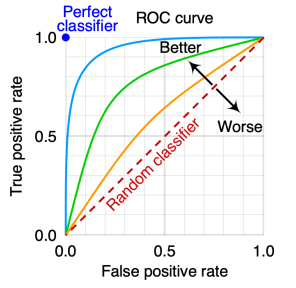
\includegraphics[width=.9\linewidth]{img/roc.png}
\end{center}


\textbf{KNN}

KNN is a classification algorithm.
KNN calculates the \(k\) nearest neighbors of it and returns the most frequent class of the \(k\) neighbors.


\textbf{KNN Algorithm}

\begin{enumerate}
\item load the training data \& test data
\item choose the value of \(k\)
\item For each test data points x\textsubscript{test}
\begin{enumerate}
\item For all training data x\textsubscript{train}, calculate the \(d(x_{test}, x_{train})\)
\begin{itemize}
\item distance metric: euclidean, Manhattan, cosine, \ldots{}
\end{itemize}
\item Sort training data in the ascending order of the distance
\item Choose the first \(k\) data points from the sorted training data
\item Choose the most frequently occurring class from the \(k\) data points as the classification result.
\end{enumerate}
\end{enumerate}


KNN can be adjusted with the numbers of neighbors (\(k\)) and the distance metric.


\textbf{Multiclass classification with linear regression}

\emph{One-vs.-rest}
Train a single classifier for each class \(c\).
The samples of class \(c\) as positive and all other samples as negative.
Apply all classifiers to an unseen sample \(x\).
The classifier reports the highest \(p\) is the class.


\emph{One-vs.-one}
Train classifiers to distinguish between each pair of classes.
Apply all classifiers to an unseen sample \(x\).
Combine the result to produce final classification.

\textbf{Unsupervised learning}

\begin{quote}
Goal: identify hidden patterns among the data.
A simple example of a structure in the data
are clusters: i.e the data points which
have some shared properties will fall into
one cluster or one alike group. ---Marko Lehmann
\end{quote}


\textbf{Clustering algorithm}

\begin{enumerate}
\item Pick \(k\) random data points (class).
\item For each of the remaining data points calculate the similarity to the \(k\) clusters.
\item The data point is assigned to the most similar class.
\end{enumerate}


\textbf{Naive k-means clustering}

k-means is a clustering algorithm.

\begin{enumerate}
\item Assume the number of clusters \(k_c\)
\item Initialize the value of the \(k\) clusters centers / mean (\(C_1\), \(C_2\), \ldots{}, \(C_{k_c}\))
\item Assignment:
\begin{enumerate}
\item Find the \emph{squared euclidean distance} between the centers and all the data points.
\item Assign each data point to the cluster of \emph{the nearest center}
\end{enumerate}
\item Update: Each cluster now potentially has a new center.
\begin{enumerate}
\item New Centres (\(C'_1, C'_2\), \ldots{}, \(C'_3\)) = Average of all the data points in the cluster.
\end{enumerate}
\item If some stopping criterions met, Done
\item Else, go to Assignment / Step 3
\end{enumerate}


\textbf{Initialization}:

\begin{itemize}
\item Run the algorithm multiple times with randomly chosen initial centers \(\rightarrow\) are the clusters stable?
\end{itemize}


\textbf{Possible Stopping Criterions}:

\begin{itemize}
\item When the centers don't changed (time-consuming)
\item The distance of data points from their centers <= threshold
\item Fixed number of iterations
\end{itemize}


\textbf{Good Solution}

In ML you execute the same algorithm multiple times with different staring parameters.
With this approach you get a better view about the whole situation.
Additional you can be sure that your parameters result in a good model.


\textbf{Scale value}

It is important that all data are in the same range.
If not the extremes (min / max) may dominate the algorithm.


\textbf{Cluster quality}

\emph{WCSS - Within-cluster sum-of-squre}: For each cluster you calculate \ref{eq:org8bb8741} and try to minimize it.
\begin{equation}
\label{eq:org8bb8741}
\sum_{i=1}^n d(C_k, x)^2
\end{equation}

\emph{Silhouette Score}
\begin{itemize}
\item \emph{a}: average intra-cluster distance
\item \emph{b}: average inter-cluster distance
\end{itemize}
\begin{equation}
  \text{Silhouette Score of a point} = \frac{b-a}{\max(a,b)}
\end{equation}

Each point has multiple \(a\) and \(b\).
For a data point \(X\) the average distance to each other data point in the cluster is \(a\).
For a data point \(X\) the average distance to each other data point in the other cluster is \(b\).


\begin{center}
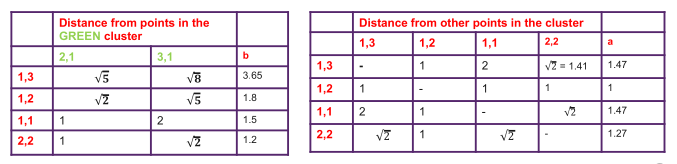
\includegraphics[width=.9\linewidth]{img/silhouette_score_a_b.png}
\end{center}

\begin{center}
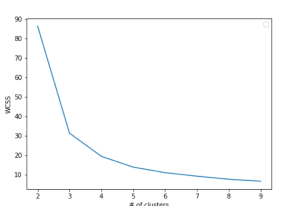
\includegraphics[width=.9\linewidth]{img/elbow_method.png}
\end{center}

\textbf{Wisdom of Crowd}

Suppose you have a very difficult question to answer.
If you don't know the answer you can search for the best suited expert, who answers your question.
But sometimes it is better to ask many random people and aggregate the answers.
This might produce the better result.
This is called the \emph{Wisdom of Crowd}.

\textbf{Ensemble}

A group of predictors is called Ensemble.
In ML you can aggregate several weak models.
If you aggregate predictors of regressors or classifiers you might get a better predictor than the best predictor!
This is a type of \href{../../../roam/20211228083830-wisdom_of_crowd.org}{Wisdom of crowd}.

\textbf{Enseble Learning}

Ensemble Learning use different models.
A model can be different in the following dimensions:
\begin{itemize}
\item algorithms
\item hyperparameters
\item training data
\end{itemize}


Different model predict a solution.
And in a vote the final prediction is chosen.

\begin{center}
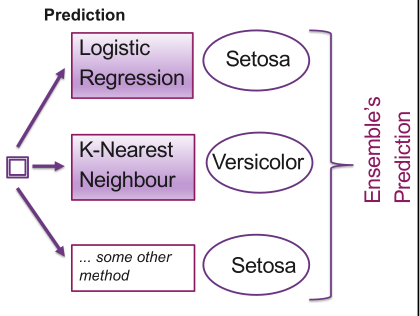
\includegraphics[width=.9\linewidth]{img/ensemble_learning_example.png}
\end{center}


\textbf{Hard / Soft Voting}

Hard and soft voting are used to decide which prediction should be used in \href{../../../roam/20211228090232-ensemble_learning.org}{Ensemble Learning}.
\begin{itemize}
\item \emph{Hard voting}: the prediction with the most votes is used
\item \emph{Soft voting}: the prediction with the highest class probability
\end{itemize}


\textbf{Bagging / Pasting}

Sampling with replacement is called \emph{Bagging} (Bootstrap Aggregating).
Sampling without replacement is called \emph{Pasting}.


\textbf{No free luch theorem}

\begin{quote}
No free lunch theorem (informal): no single machine learning algorithm is universally the best-performing algorithm for all problems
-- Marko Lehmann
\end{quote}


\textbf{Out-Of-Bag}

In Bagging some data points may be used several times.
Other data points may not be used at all.
This not seen data are called \emph{out-of-bag} (oob) data and can be used for evaluation.

\end{multicols}
\end{document}
